\documentclass[../Main.tex]{subfiles}

\begin{document}
\subsection{Plotting and analysing the data}
To get a bit of an overview of the situation the authors decided to create some plots.
\subsubsection{Plot by Day of the week}
\begin{figure}[H]
\centering
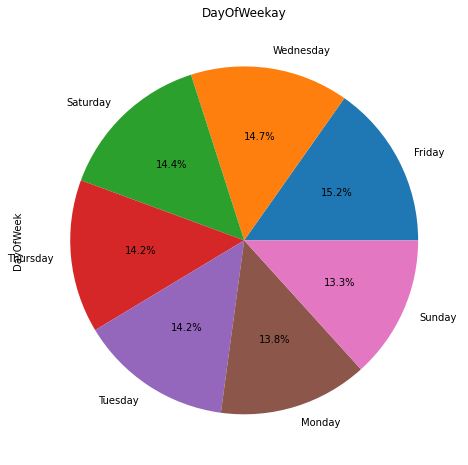
\includegraphics[width=0.3\textwidth]{Resources/DayDistribution.png}
\caption{\label{fig:DayDistribution}DayDistribution.}
\end{figure}




\subsubsection{Plot by District}

\begin{figure}[H]
\centering
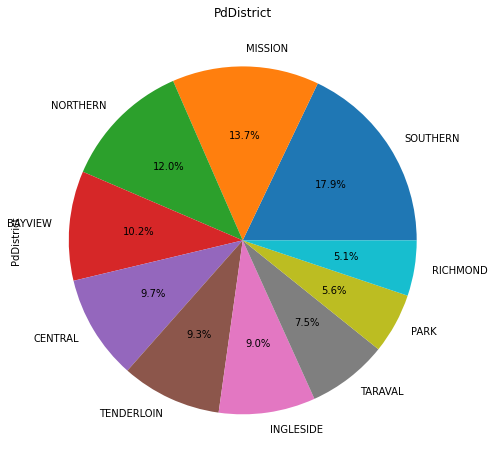
\includegraphics[width=0.3\textwidth]{Resources/DistrictDistribution.png}
\caption{\label{fig:DistrictDistribution}DistrictDistribution.}
\end{figure}

\subsubsection{Plot by the hour}

\begin{figure}[H]
\centering
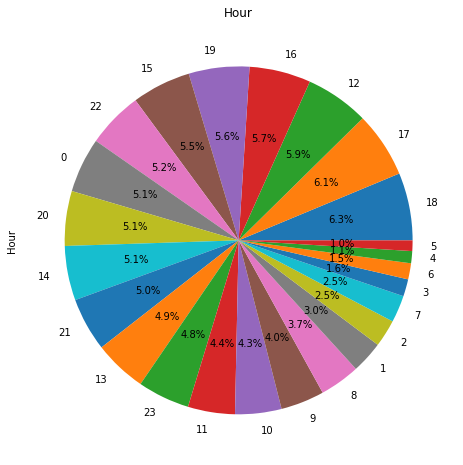
\includegraphics[width=0.3\textwidth]{Resources/HourDistribution.png}
\caption{\label{fig:HourDistribution}HourDistribution.}
\end{figure}

\subsubsection{Map of districts}
\begin{figure}[H]
\centering
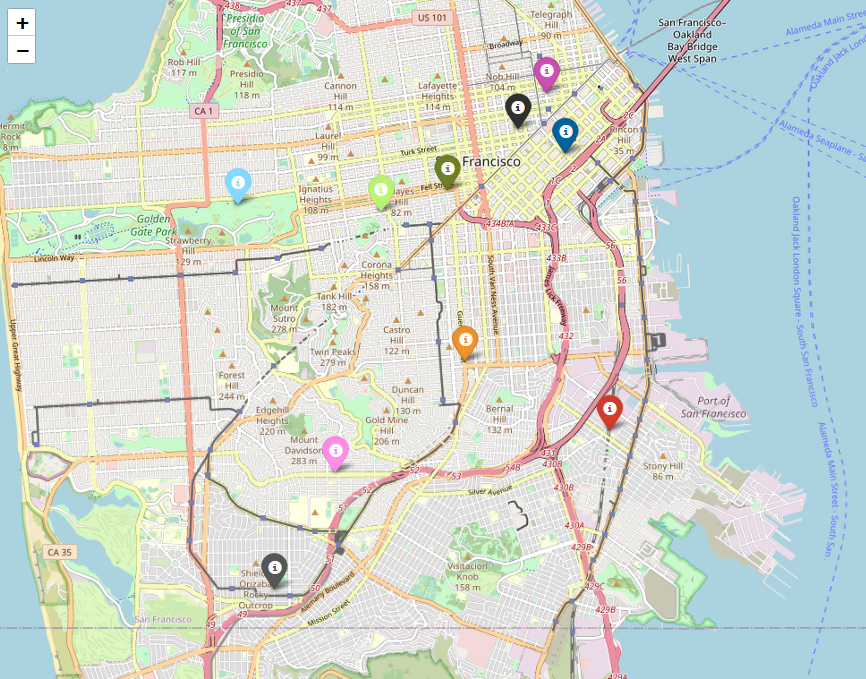
\includegraphics[width=0.3\textwidth]{Resources/MapOfDistricts.png}
\caption{\label{fig:MapOfDistricts}MapOfDistricts.}
\end{figure}

\subsubsection{Plot by Year}
\begin{figure}[H]
\centering
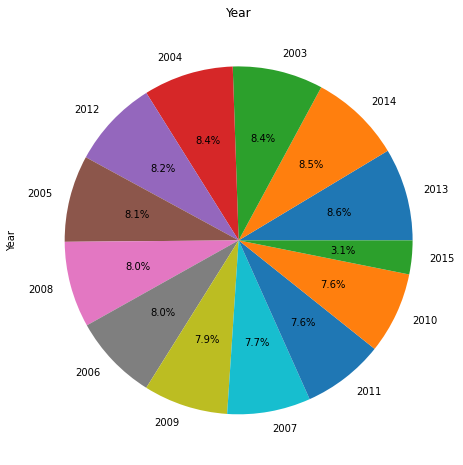
\includegraphics[width=0.3\textwidth]{Resources/YearDistribution.png}
\caption{\label{fig:YearDistribution}YearDistribution.}
\end{figure}

\subsubsection{Plot by category}

\begin{figure}[H]
\centering
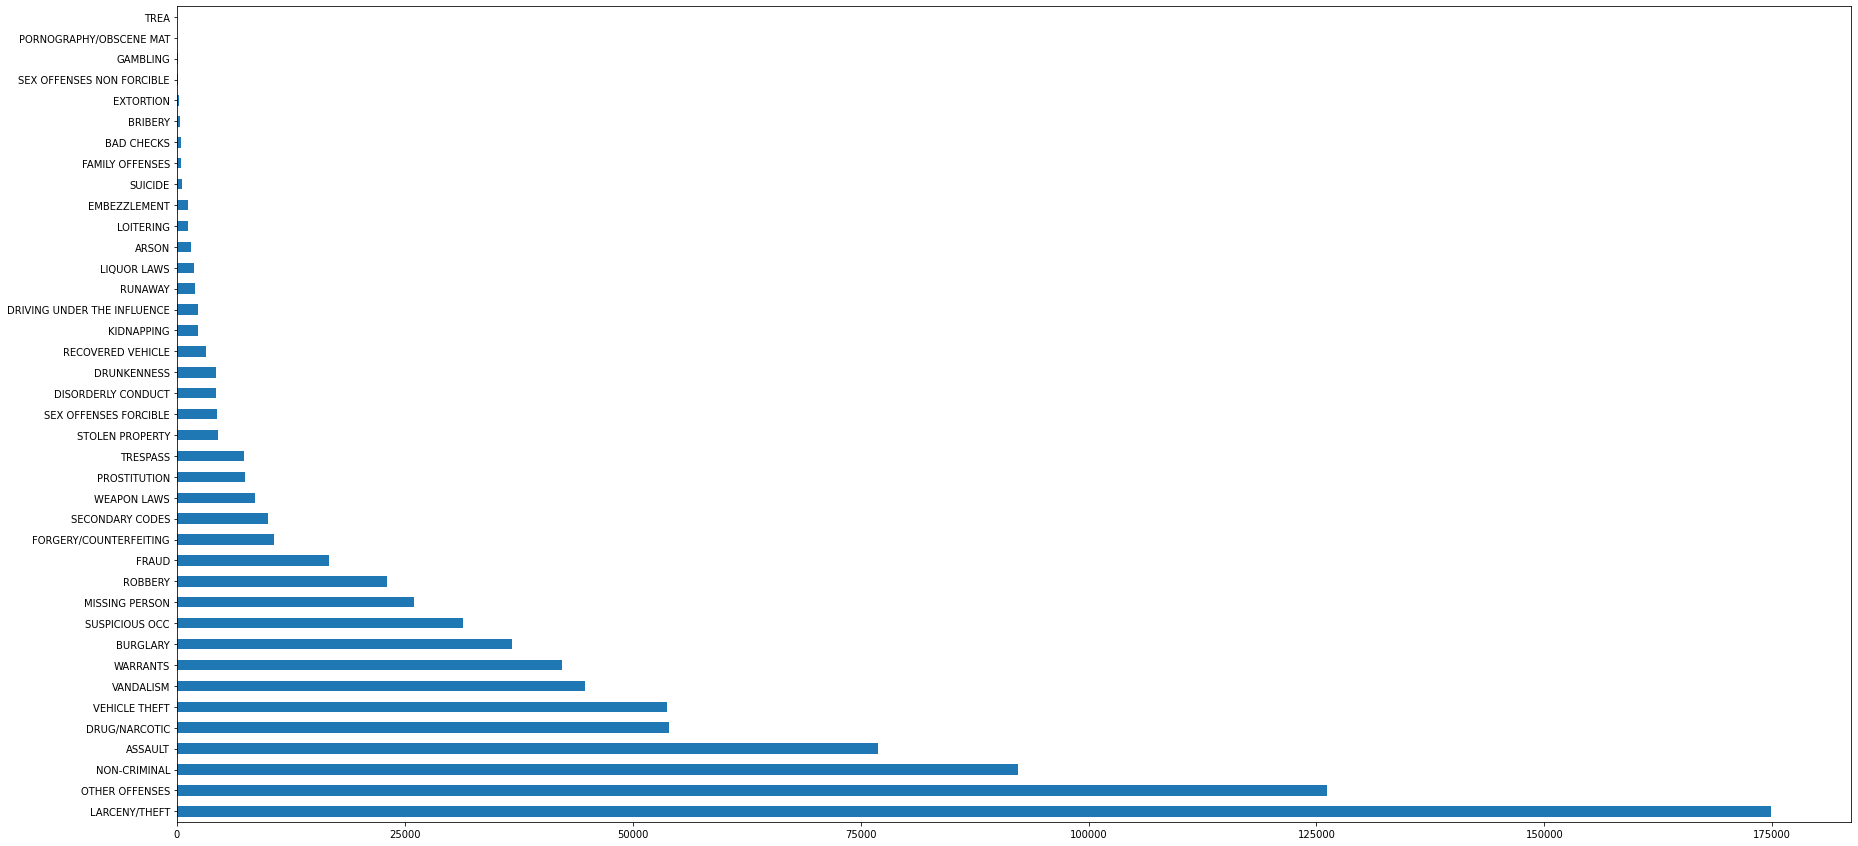
\includegraphics[width=0.3\textwidth]{Resources/CategoryDistribution.png}
\caption{\label{fig:CategoryDistribution}CategoryDistribution.}
\end{figure}




\subsubsection{Conclusion}
As one can see the crimes are relatively evenly distributed throughout the districts and dates. The only difference one can see is it depends on the hour of the day what the frequency of crimes are. Also the category samples are unbalanced.
\end{document}